\label{app:microfluidics}

\par In most BioMEMS there is fluid flow on the micrometer scale. At this scale fluid flow physics differ from fluid flow at the macro scale. Understanding and leveraging microfluidic mechanics allows for small reagent and sample volumes, multiplexing, and physic phenomenon that allow experiments and functions not possible at the macro scale. Laminar flow, diffusion, fluidic resistance, surface area to volume, and surface tension, may not be dominant in phenomenon on the macro scale, but on the micro scale become significant \cite{david_j._beebe_physics_2002}. 
%Microfluidics are discussed in further detail in appendix \ref{app:}.

\section{The Navier-Stokes Equation}

\par The Navier-Stokes formula is a partial differential equation that describes the fluid velocity given a set of boundary conditions. The Navier-Stokes equation is derived from applying Newton's second law to an infinitesimally small arbitrary control volume:
\begin{equation}
    \rho \frac{\text{D}\textbf{u}}{\text{D}t} = \sum \textbf{f},
    \label{eqn:cons_momentum}
\end{equation}

\noindent where $\rho$ is the mass density, $\textbf{u}$ is the velocity vector, $\sum \textbf{f}$ is the sum of forces applied to the control volume, and $\frac{\text{D}()}{\text{D}t}$ is the material derivative \cite{probstein_physicochemical_2005}. The material derivative is the time derivative of a function that is spatially dependent and arises from the chain rule. The material derivative of an arbitrary spatial and temporal function ($F = F(t,x,y,z)$) can be calculated as
\begin{equation}
    \frac{\text{D}F}{\text{D}t} = \frac{dF}{dt} + \frac{dF}{dx}\frac{dx}{dt} + \frac{dF}{dy}\frac{dy}{dt} + \frac{dF}{dz}\frac{dz}{dt},
\end{equation}

and can be expressed as 
\begin{equation}
    \frac{\text{D}F}{\text{D}t} = \frac{dF}{dt} + \textbf{v} \cdot \boldsymbol{\nabla}F,
\end{equation}

or in index notation as
\begin{equation}
    \frac{\text{D}F}{\text{D}t} = \frac{dF}{dt} + v_j\frac{dF}{dx_j}.
\end{equation}

\noindent The material derivative is valid for scalars and vectors.

\par Surface forces are present in many fluid systems and generally arise from pressure driven flow and viscous properties of the fluid. In general, the surface forces are expressed as the divergence of the stress tensor:
\begin{equation}
    \textbf{f}_s = \boldsymbol{\nabla} \cdot \Tau,
\end{equation}
\begin{equation}
    \textbf{f}_s = \frac{d\tau_{ij}}{dx_i},
\end{equation}

\noindent where $\textbf{f}_s$ is the surface force, and $\Tau$ and $\tau_{ij}$ are the second order stress tensor which is dependent on the type of fluid and the driving forces. For pressure driven inviscid fluids, the stress tensor and surface forces can be expressed as 
\begin{equation}
    \tau_{ij} = -p\delta_{ij},
\end{equation}
\begin{equation}
    \textbf{f}_s = - \frac{dp}{dx_j},
\end{equation}

\noindent where p is the pressure. 

\par For a viscid Newtonian fluid, the stress tensor and surface force can be expressed as \cite{probstein_physicochemical_2005}
\begin{equation}
    \tau_{ij} = -p\delta_{ij} + 2\mu(\epsilon_{ij} - \frac{1}{3}\epsilon_{kk}\delta_{ij}),
\end{equation}
\begin{equation}
    \textbf{f}_s = \frac{dp}{dx_i} + \mu \frac{d}{dx_j}(\frac{du_i}{dx_j} + \frac{du_j}{dx_i} - \frac{2}{3}\delta_{ij}\frac{du_k}{dx_k}),
    \label{eqn:viscid_newt_force}
\end{equation}

\noindent where $\epsilon_{ij}$ is the rate of strain tensor written as 
\begin{equation}
    \epsilon_{ij} = \frac{1}{2} \Big(\frac{du_i}{dx_j} + \frac{du_j}{dx_i}\Big).
\end{equation}

\noindent If the fluid is incompressible, then conservation of mass states
\begin{equation}
    \frac{du_k}{dx_k} = \boldsymbol{\nabla} \cdot \textbf{u} = 0,
    \label{eqn:incompressible_cons_mass}
\end{equation}

\noindent and equation \ref{eqn:viscid_newt_force} can be simplified to 
\begin{equation}
    \textbf{f}_s = -\frac{dp}{dx_i} + \mu \frac{d^2u_i}{dx^2_j}
\end{equation}
\begin{equation}
    \textbf{f}_s = -\boldsymbol{\nabla}p + \mu\boldsymbol{\nabla}^2\textbf{u}
    \label{eqn:viscous_pressure_force}
\end{equation}

\par Additional common forces on the control volume can include the gravitational force
\begin{equation}
    \textbf{f}_g = \rho \textbf{g},
    \label{eqn:gravity_force}
\end{equation}

\noindent where \textbf{g} is the acceleration of gravity, and for some microfluidic applications, the electroosmotic flow force (EOF)
\begin{equation}
    \textbf{f}_{EOF} = -\rho_e \boldsymbol{E},
\end{equation}

\noindent where $\boldsymbol{E}$ is the electric field vector, and $\rho_e$ is the net charge density of the electric double layer (EDL). Electric osmotic flow arises from the Coulomb force caused by the net electric charge from the electric double layer at the channel surface and the applied electric field. The electric double layer arises from the equilibrium of the solid-fluid interface \cite{kirby_micro-and_2010}. EOF results in plug flow which is characterized by a flat velocity profile in contrast to a parabolic velocity profile in pressure driven flow (figure \ref{fig:plug_vs_parabolic_flow}).

\begin{figure}[ht]
    \centering
    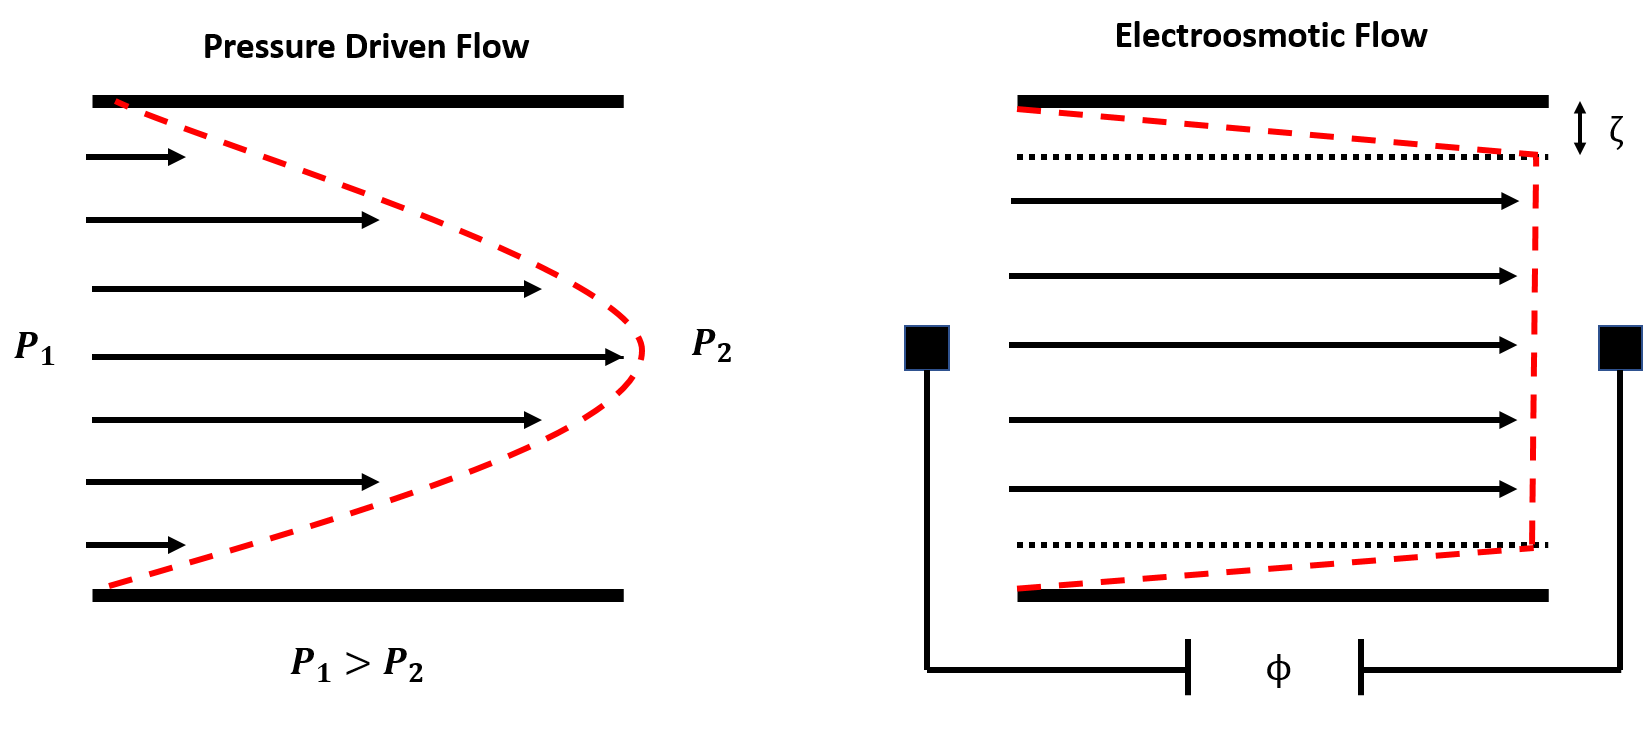
\includegraphics[width = \textwidth]{images/plugVsParabolic.png}
    \caption[Pressure driven versus electroosmotic flow profile]{Pressure driven versus electroosmotic flow profile. The pressure driven flow results in a parabolic flow profile while the electroosmotic flow with an applied voltage of $\phi$ results in a plug flow velocity profile. Near the wall of the EOF conduit in the EDL, the velocity increases until outside of the EDL there is no net charge to fight viscous forces, and the velocity profile plateus.}
    \label{fig:plug_vs_parabolic_flow}
\end{figure}

\par The most common form of the Navier-Stokes equation includes the surface forces of pressure driven Newtonian fluids with the gravitational forces, and can be expressed by combining equations \ref{eqn:cons_momentum}, \ref{eqn:viscous_pressure_force}, and \ref{eqn:gravity_force}. 
\begin{equation}
    \rho(\frac{d\textbf{u}}{dt} + \textbf{u}\cdot\boldsymbol{\nabla}\textbf{u}) = -\boldsymbol{\nabla}p + \mu\boldsymbol{\nabla}^2\textbf{u} + \rho \textbf{g}
    \label{eqn:navier_stokes}
\end{equation}

\noindent For microfluidic applications, the Navier-Stokes equation can often be simplified by assuming negligible inertial forces (Re $<<$ 2300; laminar flow) and gravitational forces allowing equation \ref{eqn:navier_stokes} to be rewritten as
\begin{equation}
        \boldsymbol{\nabla}p = \mu\boldsymbol{\nabla}^2\textbf{u}.
\end{equation}

\par Currently there is no general solution to the Navier-Stokes equation, but can be solved in specific applications with simplifying assumptions, and is widely used in computational approximations.

\section{Laminar Flow}
\par Laminar flow describes the condition where the velocity of a particle in fluid flow is not a random function of time. This is in contrast to turbulent flow which is chaotic \cite{david_j._beebe_physics_2002}. The dimensionless Reynold number can quantitatively characterize a fluid flow and is a ratio of inertial and viscous forces. The Reynold number can be expressed as
\begin{equation}
    \text{Re} = \frac{\rho v L}{\mu},
\end{equation}

\noindent where $\rho$ is the fluid density, $v$ is the characteristic fluid velocity, $\mu$ is the fluid viscosity, and $L$ is the characteristic length. In many cases, the characteristic length is the hydraulic diameter ($D_h$). The hydraulic diameter is used for fluid calculations in non-circular conduits by relating the conduit to a circular geometry in a proportion that maintains the conservation of momentum of the original conduit \cite{david_j._beebe_physics_2002}.

\par The hydraulic diameter can be expressed as ratio of cross-sectional area to conduit perimeter:
\begin{equation}
    D_h = 4 \frac{A}{P},
    \label{eqn:hydraulic_diameter}
\end{equation}

\noindent where $A$ and $P$ are the cross-sectional area and perimeter of the conduit respectively. For a cylindrical conduit, equation \ref{eqn:hydraulic_diameter} simplifies to $D_h = D_c$ where $D_c$ is the diameter of a circular cross-section. For a rectangular cross-section, the hydraulic diameter is expressed as 
\begin{equation}
    D_h = \frac{2hw}{w+h},
\end{equation}

\noindent where $h$ and $w$ are the height and width of the cross-sectional rectangle respectively. For turbulent flows, where the geometry is of lesser consequence, equation \ref{eqn:hydraulic_diameter} is a good approximation for fluid calculations, but for laminar flow, specifics of the conduit geometry is of great consequence and equation \ref{eqn:hydraulic_diameter} should be used with caution.

\par In general, flow conditions with a Reynolds number much larger than 2300 exhibit turbulent behaviours, and flow conditions with a Reynolds number much smaller than 2300 exhibit laminar flow behaviours. The laminar-turbulent transition number of 2300 is reportedly accurate for microfluidics as well \cite{david_j._beebe_physics_2002}.

\par Referring back to equation \ref{eqn:hydraulic_diameter}, since the product of characteristic length and velocity for microfluidic systems, most microfluidic flows are considered laminar. An important consequence is that separate streams that come in contact will not mix via convection, but primarily through diffusion. This phenomenom can be quantified with the dimensionless P\'eclet number (Pe), which is defined as the ratio of convection transport to diffusion transport \cite{nguyen_micromixersreview_2005}. The P\'eclet number can be expressed as 
\begin{equation}
    \text{Pe} = \frac{vL}{D}
\end{equation}

\noindent where D is the diffusion coefficient. The P\'eclet number can also be defined with the Reynolds number
\begin{equation}
    Pe = \text{Re}\;\text{Sc}
\end{equation}

\noindent where Sc is the dimensionless Schmidt number and describes the ratio of momentum diffusivity and and mass diffusivity. The Schmidt number can be calculated as
\begin{equation}
    \text{Sc} = \frac{\mu}{\rho D}
\end{equation}

\par For fluid systems where Pe is much larger than 1, the system is convection dominated and when Pe is much smaller than 1, the system is diffusion dominated. Again, the product of the characteristic velocity and length in microfluidic systems is usually very small so in BioMEMS, the system is diffusion dominated and cannot rely on convective mixing. To facilitate mixing in microfluidic systems, the device should be designed to create large surface areas between streams to expedite the diffusion process, or stimulate turbulent flow to create convective transport.


\section{Diffusion}

\par Since microfluidic flow is almost always laminar, mixing will mainly occur via diffusion (figure \ref{fig:diffusion_ilustration}) \cite{david_j._beebe_physics_2002}. Diffusion is the phenomenon where a concentration will average over a volume by Brownian motion. Fick's laws gives a quantitative description of diffusion. The first law states that the molar flux of a dissolved species is proportional to the concentration gradient of that species and can be expressed as 
\begin{equation}
    \boldsymbol{J} = -D \boldsymbol{\nabla}C,
    \label{eqn:ficks_first}
\end{equation}

\noindent where $\boldsymbol{J}$ is the molar flux of a diffusive species, $\boldsymbol{\nabla}C$ is the concentration gradient, and $D$ is a proportionality factor known as the translational diffusion constant.

\par Fick's second law arises from the continuity of mass
\begin{equation}
    \frac{dC}{dt} + \boldsymbol{\nabla} \cdot \boldsymbol{J} = 0,
\end{equation}

\noindent And by substituting in Fick's first law (equation \ref{eqn:ficks_first}), Fick's second law can be expressed as 
\begin{equation}
    \frac{dc}{dt} = D\Delta C
    \label{eqn:ficks_second}
\end{equation}

\noindent Equation \ref{eqn:ficks_second} describes the time and spatial dependencies of concentrations.

\par By examining the random walk of a particle due to Brownian motion, the mean displacement of particles can be described:
\begin{equation}
    \Big< r^2 \Big> = 2 N D t
\end{equation}

\noindent where $<r^2>$ is the squared mean displacement of a particle, $N = 1$, $2$, or $3$ for analysis in 1, 2, or 3 dimensions respectively, $t$ represents the time elapsed, and $D$ is the translation diffusion constant. 

\par The translation diffusion constant is a ratio of thermal motion and viscous resistance terms and can be generally expressed as 
\begin{equation}
    D = \frac{k_bT}{\overline{f}},
\end{equation}

\noindent where $k_b$ is the boltzman constant, $T$ is the temperature, and $\overline{f}$ is the mean friction coefficient \cite{probstein_physicochemical_2005}. The mean friction coefficient arises from the average of the translation friction tensor ($f_{ij}$) components. This tensor describes the viscous force on a particle as a function of velocity:
\begin{equation}
    F_i = f_{ij}v_j
\end{equation}

\noindent where for a rigid particle
\begin{equation}
    f_{ij} = 6\pi \mu R_{ij},
\end{equation}

\noindent where $\mu$ is the fluid viscosity, and $R_{ij}$ is the translation tensor that describes the equivalent radius. For a spherical particle, $R_{ij}$ reduces to the radius of the sphere and $f_{ij}$ becomes the viscous resistance from Stokes law. In this special case, the diffusion translation constant becomes
\begin{equation}
    D_o = \frac{k_BT}{6 \pi \mu r},
\end{equation}

and is known as the Stokes-Einstein equation. For spheroid particles where the radius depends on the orientation of the particle, the mean friction coefficient can be used since brownian motion will randomly move the particle in all directions. From the translation friction tensor, the mean friction coefficient can be described as 
\begin{equation}
    \overline{f}^{-1} = \frac{1}{3}(\frac{1}{f_1} + \frac{1}{f_2} + \frac{1}{f_3})
\end{equation}

\noindent where $f_1$, $f_2$, and $f_3$ refer to the components of the main diagonal of the translation friction tensor \cite{probstein_physicochemical_2005}. 

\begin{figure}[ht]
    \centering
    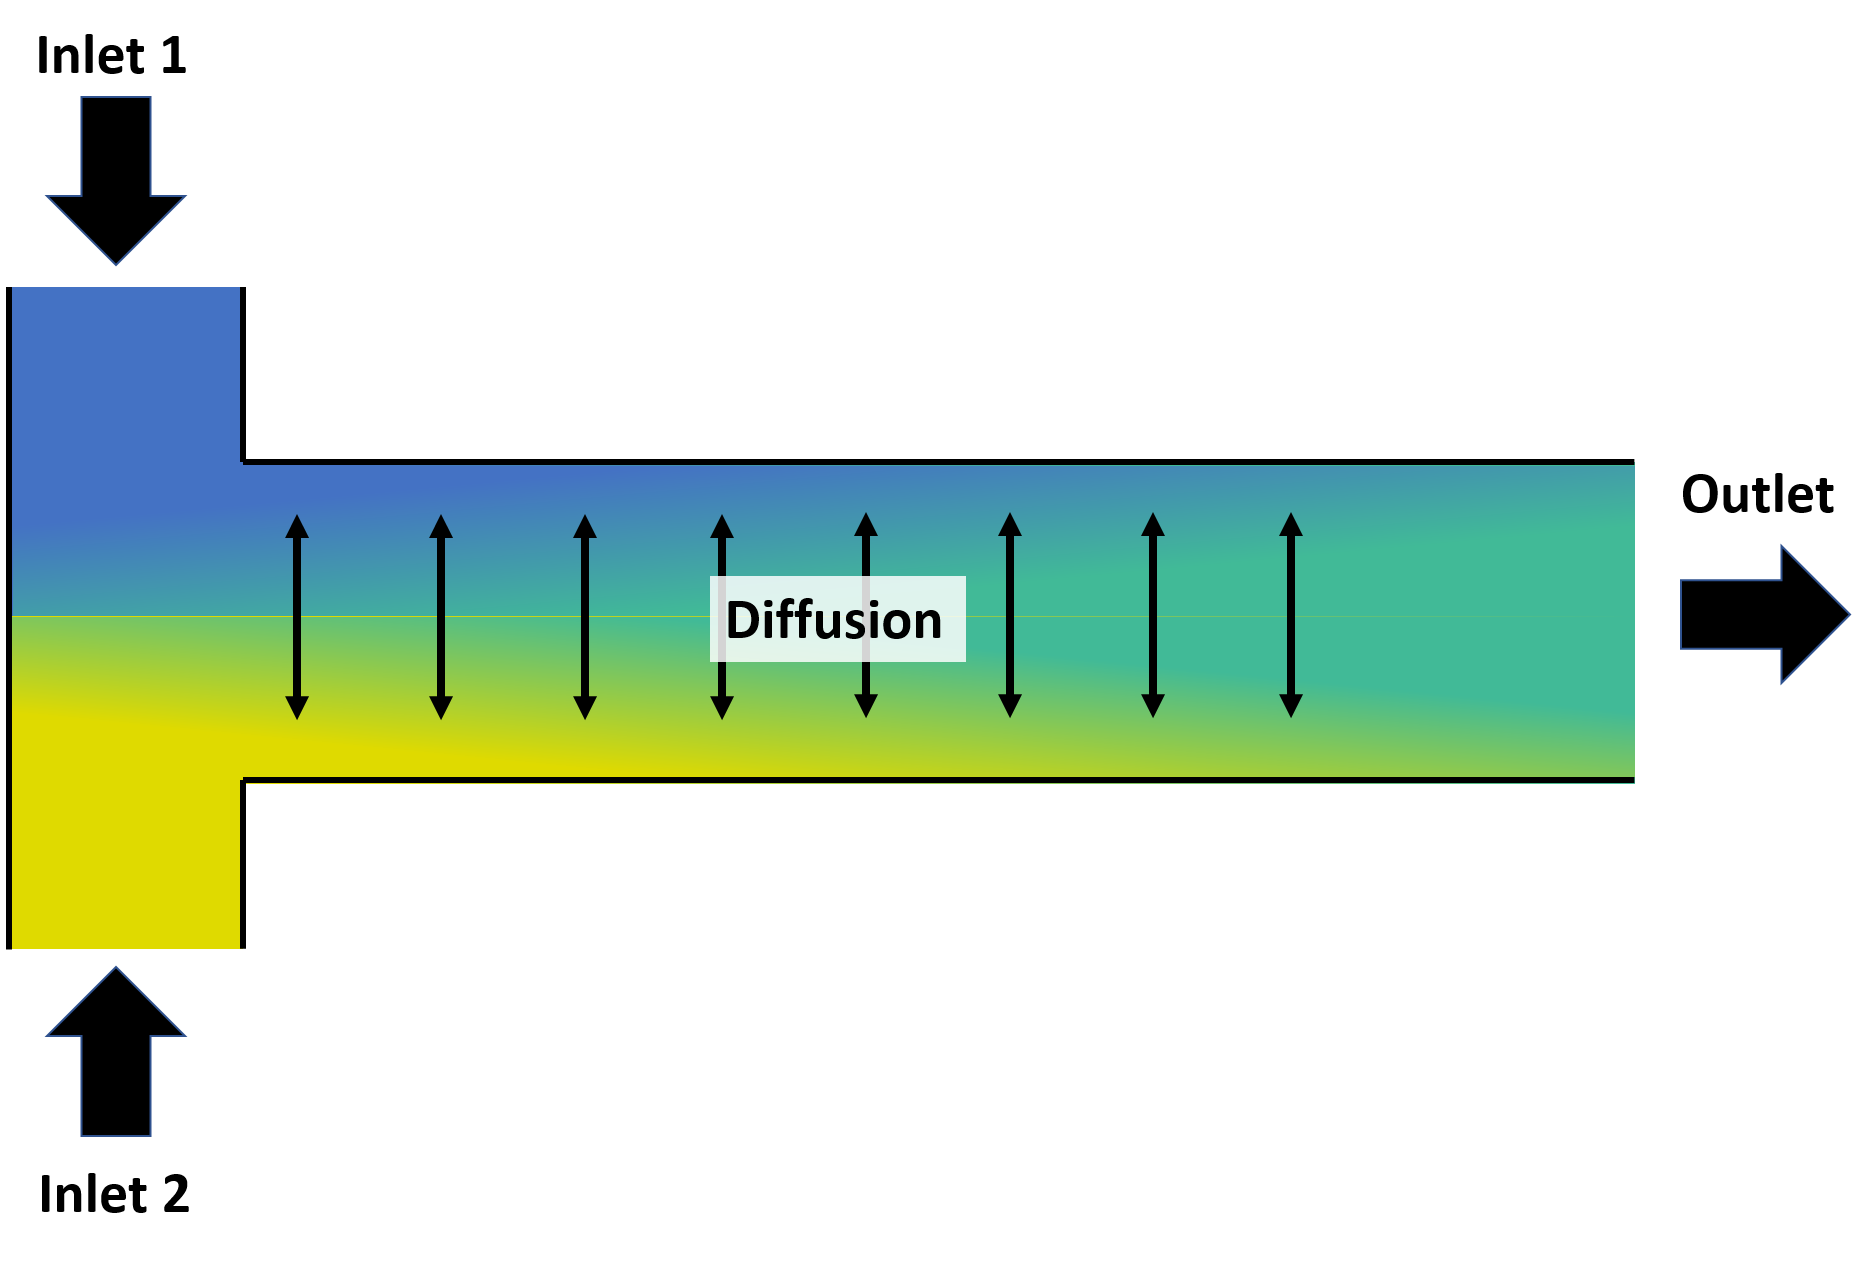
\includegraphics[width=\textwidth]{images/diffusion_illustration.png}
    \caption{Illustration of diffusion dominated transport.}
    \label{fig:diffusion_ilustration}
\end{figure} 


\section{Hydraulic Resistance}

\par Fluid resistance is a powerful analogy of fluid flow to Ohm's law where pressure is analagous to electric potential, and volumetric flow rate ($Q$) is analagous to electrical current: 
\begin{equation}
    \Delta V = I R,
    \label{eqn:ohm_analogy}
\end{equation}
\begin{equation}
    \Delta P = Q R.
    \label{eqn:ohm_fluid}
\end{equation}

\noindent In both equation \ref{eqn:ohm_analogy} and \ref{eqn:ohm_fluid} there is a quantity referred to as the resistance that resists a flow under an applied voltage or pressure. 

\par If the velocity profile is solved for from the Navier-Stokes equation and is integrated over the volume of the conduit, the volumetric flow rate as a function of applied force can be derived. In the case of pressure-driven flow of a non-compressible Newtonian fluid through a cylindrical conduit, the Hagen-Pouisuelle equation is derived, and is expressed as
\begin{equation}
    \Delta P = Q \frac{8\mu L}{\pi R_c^4}
\end{equation}

\noindent where $L$ is the length of the conduit, $R_c$ is the radius of the conduit, and $\mu$ is the viscosity. In the case of Hagen-Pouisuelle flow, the hydraulic resistance is 
\begin{equation}
    R = \frac{8\mu L}{\pi R_c^4}.
\end{equation}

\par In the case of a rectangular conduit, the hydraulic resistance can be expressed as
\begin{equation}
    R = \frac{12\mu L}{wh^3}\Bigg[1 - \frac{h}{w}\bigg( \frac{192}{\pi^5} \sum_{n=1,3,5}^\infty \frac{1}{n^5} \tanh\Big(\frac{n\pi w}{2h}\Big) \bigg) \Bigg]^{-1},
\end{equation}

\noindent where $w$ and $h$ are the cross-sectional width and height of conduit respectively \cite{david_j._beebe_physics_2002}. If the width is far greater or smaller than the width, the hydraulic resistance can be expressed by a much simpler expression \cite{david_j._beebe_physics_2002}:
\begin{equation}
    R = \frac{12 \mu L}{wh^3} 
\end{equation}

\par The Ohm's law analogy of fluid flow can be expanded to other circuit techniques such as equivalent parallel and series resistors, and Krichoff's current and voltage laws. This analogy allows for the design of complicated fluid networks at the system level.
